% id: 143-296
% book: 개념원리 공통수학1 · 16 이차방정식과 이차함수의 관계
% section: 연습문제 STEP 1
% figure: crop:fig-143-296.png
% answer: $-10$
% answer_source: 답지
% variant_level: 0 (원본 전사)
% 이 파일은 build.mjs 가 items.json 에서 만든다. 고칠 때는 items.json 을 고친다.
\smash{\raisebox{1.5mm}{\dmkichul{개념원리 공통수학1 143쪽 296번}}}
\noindent\begin{minipage}[t]{0.58\linewidth}\vspace{0pt}\raggedright 이차함수 $y=-x^2+4x-1$의 그래프와 직선 $y=ax+b$가 오른쪽 그림과 같을 때, 유리수 $a$, $b$에 대하여 $ab$의 값을 구하시오.\end{minipage}\hfill\begin{minipage}[t]{0.4\linewidth}\vspace{0pt}\centering \setlength{\dmfigw}{85.1pt}\ifdim\dmfigw>\linewidth\setlength{\dmfigw}{\linewidth}\fi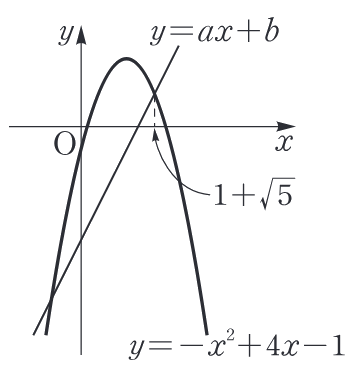
\includegraphics[width=\dmfigw]{figures/fig-143-296.png}\end{minipage}\par
